\begin{name}
	{\tenchude}
	{\tendethi}
	{\tentruong}
	{\thoigian}
\end{name}
\setcounter{ex}{0}\setcounter{bt}{0}
\TN
\Opensolutionfile{ans}[ans/ansDe2-TN1]
\begin{ex}%[Dự án K10, HKI, THPT Ngô Gia Tự năm học: 2021-2022, Nguyễn Anh Quốc]%[0D1N1-1]
	Cho mệnh đề $A:$ \lq\lq  $\forall x\in \mathbb{R}, x^2-x+7\ne 0$\rq\rq. Mệnh đề phủ định của $A$ là
	\choice
	{\True $\exists x \in \mathbb{R},x^2-x+7=0$}
	{$\exists x \in \mathbb{R},x^2-x+7\ge0$}
	{$\forall x \in \mathbb{R},x^2-x+7=0$}
	{$\exists  x \in \mathbb{R},x^2-x+7>0$}
	\loigiai{
		Mệnh đề phủ định của mệnh đề $A$ là  $\overline{A}:$ \lq\lq  $\exists x \in \mathbb{R},x^2-x+7=0$\rq\rq.
	}
\end{ex}

\begin{ex}%[0D1H1-3]
	Mệnh đề nào sau đây là phủ định của mệnh đề \lq\lq  Mọi động vật đều di chuyển\rq\rq?
	\choice
	{Mọi động vật đều không di chuyển}
	{Mọi động vật đều đứng yên}
	{\True Có ít nhất một động vật không di chuyển}
	{Có ít nhất một động vật di chuyển}
	\loigiai{
		Phủ định của mệnh đề \lq\lq  Mọi động vật đều di chuyển\rq\rq là mệnh đề \lq\lq  Có ít nhất một động vật không di chuyển\rq\rq.}
\end{ex}

\begin{ex}%[Đề kiểm tra HK1-Chuyên Thoại Ngọc Hầu, An Giang, 2018]%[Huỳnh Đức Vũ, dự án 0-HK1-161718]%[0D1N2-1]
	Cho tập hợp $B=\left\{\left. n\in{\mathbb{N}^*}\right|3<n^2<100\right\}$. Số phần tử của $B$ là
	\choice
	{$6$}
	{$7$}
	{\True $8$}
	{$5$}
	\loigiai{
		Ta có $3<n^2<100$ $\Leftrightarrow 2\le n\le 9$ (do $n\in{\mathbb{N}^*}$).\\
		Vậy tập hợp $B$ có $8$ phần tử.
	}
\end{ex}

\begin{ex}%[TN hóa]%[Duong Xuan Loi]%[0D1H3-3]
	Lớp $10$A có $24$ bạn tham gia thi đấu bóng đá và cầu lông, trong đó có $16$ bạn thi đấu bóng đá và $11$ bạn thi đấu cầu lông. Giả sử các trận bóng đá và cầu lông không tổ chức đồng thời. Hỏi có bao nhiêu bạn lớp $10$A tham gia thi đấu cả bóng đá và cầu lông?
	\choice
	{\True $3$}
	{$24$}
	{$11$}
	{$16$}
	\loigiai{
		Gọi $A$ là tập hợp các bạn tham gia thi đấu bóng đá $\Rightarrow n(A)=16$.\\
		Gọi $B$ là tập hợp các bạn tham gia thi đấu cầu lông $\Rightarrow n(B)=11$.\\
		Do đó $A\cap B$ là số bạn tham gia thi đấu cả bóng đá và cầu lông.\\
		Ta có $n(A \cup B)=n(A)+n(B)-n(A \cap B)\Rightarrow n(A \cap B)=n(A)+n(B)-n(A \cup B)=16+11-24=3$.
	}
\end{ex}

\begin{ex}%[Dự án Giảng 10-11 Nhóm Toán & LaTex, Lê Minh Thiện Anh]%[0D1H3-5]
	\immini{
		Cho hai tập hợp $A$ và $B$ được biểu diễn bằng sơ đồ Ven như hình vẽ bên. Phần tô đậm là biểu diễn của tập hợp nào dưới đây?
		\choice
		{$B\setminus A$}
		{$A \cup B$}
		{$A \cap B$}
		{\True $A\setminus B$}
	}
	{
		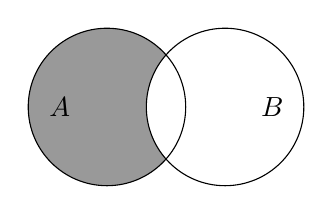
\begin{tikzpicture}
			\fill[fill=gray!80] (0,0) circle (1cm);
			\fill[fill=white] (1.5,0) circle (1cm);
			\draw (0,0) circle (1cm) (1.5,0) circle (1cm);
			\draw (-0.6,0) node {$A$} (2.1,0) node {$B$};
		\end{tikzpicture}
	}
	\loigiai{
		Phần tô đậm là biểu diễn của tập hợp $A\setminus B$.
	}
\end{ex}

\begin{ex}%[0-HK1-CTST-4-2324]%[VN-MT-9, Phúc Hậu]%[0D2N1-1]
	Cặp số $(3;-1)$ là nghiệm của bất phương trình nào dưới đây?
	\choice
	{$x-5y\leq 2$}
	{$-2x+5y-3 > 0$}
	{$2-3y\leq 0$}
	{\True $2x-7y\leq 0$}
	\loigiai{
		Vì $2\cdot3-7\cdot1\le0$ nên cặp số $(3;-1)$ là nghiệm của bất phương trình $2x-7y\leq 0$.
	}
\end{ex}

\begin{ex}%[Mức 2]%[Đỗ Đường Hiếu]%[0D2H1-2]
	\immini{
		Miền nghiệm của bất phương trình nào sau đây được biểu diễn bởi nửa mặt phẳng không bị gạch ở hình vẽ? (kể cả bờ là đường thẳng)
		\choice
		{\True $3x+2y+6\ge 0$}
		{$3x-2y+6\le 0$}
		{$2x+y+6\ge 0$}
		{$3x+2y+6\le 0$}
	}
	{
		\begin{tikzpicture}[scale=0.7, font=\footnotesize, line join=round, line cap=round,>=stealth]
			\def\a{-1.5} \def\b{-3} % Hệ số
			\def\xmin{-4} \def\xmax{2}
			\def\ymin{-4.5} \def\ymax{2}
			\draw[->] (\xmin,0)--(\xmax,0) node [below]{$x$};
			\draw[->] (0,\ymin)--(0,\ymax) node [left]{$y$};
			\node at (0,0) [below left]{$O$};
			\draw[smooth,samples=300,domain=-3.34:1] plot(\x,{\a*(\x)+\b});
			\fill[pattern=north east lines,opacity=0.5] (-4,-4.5)--(1,-4.5)--(-3.34,2)--(-4,2)--cycle;
			\fill (0,0) circle (1.0pt) (-2,0) circle (1.0pt)node[above right]{$-2$} (0,-3) circle (1.0pt)node[right]{$-3$};
		\end{tikzpicture}
	}
	\loigiai{
		Đường thẳng trong hình đi qua $A(-2;0)$ và $B(0;-3)$ có dạng $ (d)\colon y=ax+b $.\\
		Ta có $\heva{&-2a+b=0\\&0+b=-3}\Leftrightarrow \heva{&a=-\dfrac{3}{2}\\&b=-3.}$\\
		Vậy $ (d)\colon y=-\dfrac{3}{2}x-3\Leftrightarrow 3x+2y+6=0$.\\
		Thay tọa độ điểm $O(0;0)$ vào ta có $3\cdot0+2\cdot0+6=6\ge0$.\\
		Vậy miền nghiệm của bất phương trình được biểu diễn bởi nửa mặt phẳng không bị gạch ở hình vẽ là $3x+2y+6\ge 0$.
	}
\end{ex}

\begin{ex}%[De-chuan-hoa-so-8]%[Duong Xuan Loi]%[0D2N2-1]
	Trong các hệ sau, hệ nào không phải là hệ bất phương trình bậc nhất hai ẩn?
	\choice
	{$\heva{&y>0 \\& x-4 \leq 1}$}
	{\True $\heva{&x+y=-2 \\& x-y=5}$}
	{$\heva{&x+y>0 \\& x>1}$}
	{$\heva{&2 x+3 y>10 \\ &x-4 y<1}$}
	\loigiai{
		$\heva{&x+y=-2 \\& x-y=5}$ là hệ phương trình bậc nhất hai ẩn nên không phải là hệ bất phương trình bậc nhất hai ẩn.
	}
\end{ex}

\begin{ex}%[Đề HK1, Lê Quý Đôn, HCM, 23 - 24]%[Trần Hoà, 10-11EX-HK1-2324]%[0D2H2-2]
	Biểu thức $F(x;y)=x+3y-1$ đạt giá trị lớn nhất với điều kiện $\heva{&x+2y\le 2\\&x\ge 0\\&y\ge 0}$ tại điểm có toạ độ là
	\choice
	{$(0;0)$}
	{$(2;0)$}
	{$(0;2)$}
	{\True $(0;1)$}
	\loigiai
	{Ta thấy điểm $(0;2)$ có toạ độ không thoả mãn hệ bất phương trình điều kiện và các điểm còn lại có toạ độ thoả mãn.\\
		Với $(0;0)$, ta có $F(0;0)=-1$.\\
		Với $(2;0)$, ta có $F(2;0)=1$.\\
		Với $(0;1)$, ta có $F(0;1)=2$.\\
		Vậy tại điểm $(0;1)$ thì $F(x;y)$ đạt giá trị lớn nhất.}
\end{ex}

\begin{ex}%[Dự án EX-10-11-Chuẩn hóa]%[Hoàng Thanh Phương]%[0H4N2-1]
	Cho tam giác $ABC$, mệnh đề nào là đúng?
	\choice
	{$a^2=b^2+c^2-ac\cos A$}
	{$a^2=b^2+c^2+2bc\cos A$}
	{\True $a^2=b^2+c^2-2bc\cos A$}
	{$a^2=b^2+c^2+bc\cos A$}
	\loigiai{Theo định lí cosin ta có $a^2=b^2+c^2-2bc\cos A$.}
\end{ex}

\begin{ex}%[De-chuan-hoa-so-16]%[Mui Doan]%[0H4N2-2]
	Cho tam giác $ABC$, có độ dài ba cạnh là $BC=a$, $AC=b$, $AB=c$. Gọi $R$ là bán kính đường tròn ngoại tiếp tam giác và $S$ là diện tích tam giác đó Mệnh đề nào sau đây đúng?
	\choice
	{\True $S=\dfrac{abc}{4R}$}
	{$S=\dfrac{abc}{4R}$}
	{$S=\dfrac{R}{4abc}$}
	{$S=\dfrac{ac}{4R}$}
	\loigiai{
		Ta có $S=\dfrac{abc}{4R}$.
	}
\end{ex}

\begin{ex}%[BG12-3in1, Nguyễn Xuân Bảo-Phạm Ngọc Trung]%[0H4H2-1]
	Tam giác $ ABC $ có $ AC=3\sqrt{3},AB=3 $ và $ BC=6. $ Số đo góc $ \widehat{ABC} $ bằng
	\choice
	{\True $ 60^{\circ} $}
	{$ 45^{\circ} $}
	{$ 30^{\circ} $}
	{$ 120^{\circ} $}
	\loigiai{
	Ta có	$ \cos\widehat{ABC}=\dfrac{AB^2+BC^2-AC^2}{2\cdot AB\cdot BC}=\dfrac{1}{2} \Rightarrow \widehat{ABC}=60^{\circ}$.
	}

\end{ex}

\begin{ex}%[De-chuan-hoa-so-6]%[Đình Nguyên]%[0H4H1-2]
	Cho góc $\alpha\left(0^\circ<\alpha<180^\circ\right)$ thoả mãn $\sin \alpha-\cos \alpha=0$. Giá trị của  $\tan \alpha$ là?
	\choice
	{$0$}
	{$\sqrt{2}$}
	{$\dfrac{\sqrt{2}}{2}$}
	{\True $1$}
	\loigiai{
		Ta có $\sin \alpha-\cos \alpha=0 \Rightarrow \sin \alpha =\cos \alpha \Rightarrow \tan \alpha=1$.
	}

\end{ex}

\begin{ex}%[0-HK1-KN-1-PhanDinhPhung-HaNoi-2324]%[VN-MT-6, VM019]%[0H5N1-3]
	Cho điểm $M$ là trung điểm của đoạn thẳng $AB$ ($A$ không trùng với $B$). Hệ thức nào sau đây là đúng?
	\choice
	{$\overrightarrow{MA}=\overrightarrow{MB}$}
	{$\overrightarrow{AM}=\overrightarrow{AB}$}
	{$\overrightarrow{AM}=\overrightarrow{BM}$}
	{\True $\overrightarrow{AM}=\overrightarrow{MB}$}
	\loigiai{
		$M$ là trung điểm của đoạn thẳng $AB$ nên $\overrightarrow{AM}=\overrightarrow{MB}$.
	}
\end{ex}

\begin{ex}%[De-chuan-hoa-so-8]%[Duong Xuan Loi]%[0H5N2-2]
	Cho các điểm phân biệt $A$, $B$, $C$. Đẳng thức nào sau đây đúng?
	\choice
	{\True $\overrightarrow{AB}=\overrightarrow{CB}+\overrightarrow{AC}$}
	{$\overrightarrow{AB}=\overrightarrow{BC}+\overrightarrow{AC}$}
	{$\overrightarrow{AB}=\overrightarrow{BC}+\overrightarrow{CA}$}
	{$\overrightarrow{AB}=\overrightarrow{CA}+\overrightarrow{BC}$}
	\loigiai{
		Mệnh đề đúng là $\overrightarrow{AB}=\overrightarrow{CB}+\overrightarrow{AC}$.
	}
\end{ex}

\begin{ex}%[0H5H2-2]%[CTST-Lop 10-On-tap-cuoi-hoc-ki-1-De-6]%[Trần Hưng]
	Cho ba điểm $A$, $B$, $C$ phân biệt. Khẳng định nào sau đây đúng?
	\choice
	{\True $\overrightarrow{AB}+\overrightarrow{BC}=\overrightarrow{AC}$}
	{$\overrightarrow{BA}+\overrightarrow{BC}=\overrightarrow{AC}$}
	{$\overrightarrow{AB}-\overrightarrow{AC}=\overrightarrow{BC}$}
	{$\overrightarrow{CA}+\overrightarrow{BA}=\overrightarrow{CB}$}
	\loigiai{
		Ta có $\overrightarrow{AB}+\overrightarrow{BC}=\overrightarrow{AC}$ đúng (quy tắc $3$ điểm).
	}
\end{ex}

\begin{ex}%[0H5H3-2]%[KNTT - Lớp 10 - Ôn tập cuối học kì 1 - Đề 2]%[TanNguyen]
	Cho tam giác $A B C$, gọi $M$ là điểm thuộc cạnh $B C$ sao cho $B M=3 M C$. Khẳng định nào dưới đây đúng?
	\choice
	{\True $\overrightarrow{A M}=\dfrac{1}{4} \overrightarrow{A B}+\dfrac{3}{4} \overrightarrow{A C}$}
	{$\overrightarrow{A M}=\dfrac{2}{3} \overrightarrow{A B}+\dfrac{1}{3} \overrightarrow{A C}$}
	{$\overrightarrow{A M}=\dfrac{3}{4} \overrightarrow{A B}+\dfrac{1}{4} \overrightarrow{A C}$}
	{$\overrightarrow{A M}=\dfrac{5}{4} \overrightarrow{A B}+\dfrac{3}{4} \overrightarrow{A C}$}
	\loigiai
	{
		Ta có $\overrightarrow{A M}=\overrightarrow{A B}+\overrightarrow{B M}=\overrightarrow{A B}+\dfrac{3}{4} \overrightarrow{B C}=\overrightarrow{A B}+\dfrac{3}{4}(\overrightarrow{A C}-\overrightarrow{A B})=\dfrac{1}{4} \overrightarrow{A B}+\dfrac{3}{4} \overrightarrow{A C}$.
	}
\end{ex}

\begin{ex}%[Dự án Form mới 12/4/6-HK1 Lớp 10-11]%[VN-MT-6, Võ NGuyên Thạch]%[THPT TÂN TÚC-TP HCM]%[0H5N4-1]
	Cho $\overrightarrow{a}$ và $\overrightarrow{b}$ là hai vectơ đều khác vectơ $\overrightarrow{0}$. Trong các kết quả sau đây, hãy chọn kết quả đúng.
	\choice
	{$\overrightarrow{a} \cdot \overrightarrow{b}=0$}
	{$\overrightarrow{a} \cdot \overrightarrow{b}=-\left|\overrightarrow{a}\right|\cdot\left|\overrightarrow{b}\right|\cdot \cos\left(\overrightarrow{a}, \overrightarrow{b}\right)$}
	{$\overrightarrow{a} \cdot \overrightarrow{b}=\left|\overrightarrow{a}\right|\cdot\left|\overrightarrow{b}\right|$}
	{\True $\overrightarrow{a} \cdot \overrightarrow{b}=\left|\overrightarrow{a}\right|\cdot\left|\overrightarrow{b}\right|\cdot \cos\left(\overrightarrow{a}, \overrightarrow{b}\right)$}
	\loigiai{
		Ta có $\overrightarrow{a} \cdot \overrightarrow{b}=\left|\overrightarrow{a}\right|\cdot\left|\overrightarrow{b}\right|\cdot \cos\left(\overrightarrow{a}, \overrightarrow{b}\right)$.
	}
\end{ex}

\begin{ex}%[Mức 2]%[Dự án Giảng 10-11 Nhóm Toán & LaTex, Lê Minh Thiện Anh]%[0H5H4-2]
	Trong mặt phẳng với hệ tọa độ $Oxy$, cho tam giác $ABC$ với $A(1;-1)$, $B(4;2)$ và $C(4;-2)$. Hỏi góc $\widehat{ABC}$ có số đo độ bằng bao nhiêu?
	\choice
	{$30^{\circ}$}
	{\True$45^{\circ}$}
	{$60^{\circ}$}
	{$90^{\circ}$}
	\loigiai{Ta có $\overrightarrow{BA}=(-3;-3)\Rightarrow BA=3\sqrt{2}$.\\
	$\overrightarrow{BC}=(0;-4)\Rightarrow BC=4$.\\
	$\cos\widehat{ABC}=\cos\left(\overrightarrow{BA},\overrightarrow{BC}\right)=\dfrac{\overrightarrow{BA}\cdot \overrightarrow{BC}}{BA\cdot BC}=\dfrac{12}{3\sqrt{2}\cdot 4}=\dfrac{1}{\sqrt{2}}\Rightarrow \widehat{ABC}=45^{\circ}$
	}
\end{ex}

\begin{ex}%[0D8N1-1]%[Dự án đề kiểm tra Toán 10 HKII NH23-24- Đoàn Thanh Phong]%[THPT Thiệu Hóa - Thanh Hóa]
	Trong một trường THPT, khối $10$ có $280$ học sinh nam, $325$ học sinh nữ. Nhà trường cần chọn một học sinh đi dự dạ hội của học sinh tỉnh. Hỏi nhà trường có bao nhiêu cách chọn?
	\choice
	{\True $605$}
	{$325$}
	{$280$}
	{$45$}
	\loigiai{
		Số cách chọn $1$ học sinh từ các học sinh khối $10$ là $280+325=605$ cách.
	}
\end{ex}

\begin{ex}%[0D8H1-3]%[Dự án đề kiểm tra Toán 10 HKII NH23-24- Trần Văn Hùng]%[THPT Nam Lý- Hà Nam]
	Từ thành phố A đến thành phố B có $3$ con đường, từ thành phố A đến thành phố C có $2$ con đường, từ thành phố B đến thành phố D có $2$ con đường, từ thành phố C đến thành phố D có $3$ con đường, không có con đường nào nối từ thành phố C đến thành phố B. Hỏi có bao nhiêu 	con đường đi từ thành phố A đến thành phố D?
	\choice
	{$18$}
	{\True $12$}
	{$6$}
	{$36$}
	\loigiai{
		Để đi từ thành phố A đến thành phố D ta có $2$ cách.
		\begin{itemize}
			\item Cách 1. Đi từ A đến B và đi từ B đến D.\\
			      Số cách đi là $3\cdot 2=6$.
			\item Cách 2. Đi từ A đến C và đi từ C đến D.\\
			      Số cách đi là $2\cdot 3=6$.
		\end{itemize}
		Vậy có $6+6=12$ cách đi từ thành phố A đến thành phố D.
	}
\end{ex}

\begin{ex}%[BG - 10 New - 3in1, Nguyễn Văn Cường (Cường NV)]%[0D8H1-2]
	Từ các chữ số $1$, $5$, $6$, $7$ có thể lập được bao nhiêu số tự nhiên có $4$ chữ số (không nhất thiết phải khác nhau)?
	\choice
	{$324$}
	{\True $256$}
	{$248$}
	{$124$}
	\loigiai{Gọi số cần tìm có dạng $\overline{abcd}$ với $(a,b,c,d)\in A=\{1;5;6;7\}$\\.
		Vì số cần tìm có $4$ chữ số không nhất thiết khác nhau nên
		\begin{itemize}
			\item $a$ được chọn từ tập $A$ (có $4$ phần tử) nên có $4$ cách chọn.
			\item $b$ được chọn từ tập $A$ (có $4$ phần tử) nên có $4$ cách chọn.
			\item $c$ được chọn từ tập $A$ (có $4$ phần tử) nên có $4$ cách chọn.
			\item $d$ được chọn từ tập $A$ (có $4$ phần tử) nên có $4$ cách chọn.
		\end{itemize}
		Như vậy, ta có $4\cdot 4\cdot 4\cdot 4=256$ số cần tìm.}
\end{ex}

\begin{ex}%[0D8N2-1]%[Dự án đề kiểm tra Toán 10 HKII NH23-24- Đoàn Thanh Phong]%[THPT Thiệu Hóa - Thanh Hóa]
	Khẳng định nào sau đây là \textbf{sai}?
	\choice
	{$\mathrm{C}_n^k=\mathrm{C}_n^{n-k}$}
	{$P_n=n!$}
	{$\mathrm{A}_n^k=\mathrm{C}_n^k\cdot k!$}
	{\True $\mathrm{C}_n^k=\dfrac{k!}{n!(n-k)!}$}
	\loigiai
	{
		Ta có $\mathrm{C}_n^k=\dfrac{n!}{k!(n-k)!}$ nên khẳng định $\mathrm{C}_n^k=\dfrac{k!}{n!(n-k)!}$ là sai.
	}
\end{ex}

\begin{ex}%[0D8H2-3]%[Dự án đề kiểm tra Toán khối 10 HK2-NH23-24-Đợt 15-Dương Công Tạo]%[THPT Đặng Huy Trứ - Huế]
	Cho các chữ số $1,3,5,8$. Có thể lập được bao nhiêu số tự nhiên có $4$ chữ số từ các chữ số đã cho?
	\choice
	{$324$}
	{$265$}
	{$256$}
	{\True $24$}
	\loigiai{
		Số tự nhiên có $4$ chữ số từ các chữ số $1,3,5,8$ là một hoán vị của $4$ phần tử.\\
		Vậy có $4!=24$ (số).
	}
\end{ex}

\begin{ex}%[0D8N3-2]
	Tìm hệ số của $x^2$  trong khai triển biểu thức $(7x + 5)^{3}$
	\choice
	{$343$}
	{$525$}
	{\True $735$}
	{$125$}
	\loigiai{
		Ta viết khai triển biểu thức như sau
		\begin{eqnarray*}
			(7x + 5)^{3} &=& \mathrm{C}_3^0(7x)^3 + \mathrm{C}_3^1(7x)^25^1 + \mathrm{C}_3^2(7x)^15^2 + \mathrm{C}_3^3(7x)^05^3\\
			&=& 343x^3 + 735x^2 + 525x + 125.
		\end{eqnarray*}
		Suy ra hệ số của $x^2$  trong khai triển là $735$.
	}
\end{ex}

\begin{ex}%[0D8H3-3]%[tex hóa đề ck2 - form 2025 - đợt 2 - Nguyễn Hữu Thiện]
	Trong khai triển nhị thức $(2a-b)^5$, hệ số của số hạng thứ $3$ là
	\choice
	{$-80 $}
	{\True$80$}
	{$-10$}
	{$10$}
	\loigiai{Ta có
		\begin{eqnarray*}
			(2a-b)^5 &=& C_5^0 \cdot(2a)^5+C_5^1(2a)^4(-b)+C_5^2(2a)^3(-b)^2+\ldots\\
			&=&C_5^0 \cdot 2^5a^5-C_5^12^4a^4 b+C_5^22^3a^3b^2-\ldots
		\end{eqnarray*}
		Hệ số của số hạng thứ ba là $C_5^2 \cdot 2^3=80$.
	}
\end{ex}

\begin{ex}%[0H9N1-3]%[Dự án đề kiểm tra Toán 10 HKII NH23-24- Trần Văn Hùng]%[THPT Nam Lý- Hà Nam]
	Trong mặt phẳng tọa độ $Oxy$, tọa độ của véc-tơ $\overrightarrow{a}=3\overrightarrow{i}-5\overrightarrow{j}$ là
	\choice
	{$\overrightarrow{a}=(3;5)$}
	{\True $\overrightarrow{a}=(3;-5)$}
	{$\overrightarrow{a}=(-3;5)$}
	{$\overrightarrow{a}=(-5;3)$}
	\loigiai{
		Ta có $\overrightarrow{a}=(3;-5)$.
	}
\end{ex}

\begin{ex}
	Trung điểm $M$ của đoạn thẳng $AB$ có tọa độ là
	\choice
	{\True $\left(\dfrac{x_A+x_B}{2};\dfrac{y_A+y_B}{2}\right)$}
	{$\left(\dfrac{x_A-x_B}{2};\dfrac{y_A-y_B}{2}\right)$}
	{$\left(\dfrac{x_A+x_B}{3};\dfrac{y_A+y_B}{3}\right)$}
	{$(x_A-x_B;y_A-y_B)$}
\end{ex}

\begin{ex}%[0H9H1-3]%[KNTT - Lớp 10 - Ôn tập cuối học kì 1 - Đề 5]%[Phạm Hải Dương]
	Trong hệ tọa độ $Oxy$, cho điểm $A(2;-3)$, $B(3;4)$. Tìm tọa độ điểm $M$ thuộc trục hoành sao cho $A$, $B$, $M$ thẳng hàng.
	\choice
	{\True $M\left(\dfrac{17}{7}; 0\right)$}
	{$M(4; 0)$}
	{$M\left(\dfrac{5}{3}; 0\right)$}
	{$M(1; 0)$}
	\loigiai{
		Ta có $M$ thuộc trục hoành nên $M(x;0)$. \\
		Khi đó $\overrightarrow{AM} = (x-2; 3)$, $\overrightarrow{AB} = (1; 7)$.\\
		Để $A$, $B$, $M$ thẳng hàng thì $\overrightarrow{AM}$ và $\overrightarrow{AB}$ cùng phương hay $\dfrac{x-2}{1} = \dfrac{3}{7} \Leftrightarrow x = \dfrac{17}{7}$.\\
		Vậy $M\left(\dfrac{17}{7}; 0\right)$.
	}
\end{ex}

\begin{ex}%[0-HK1-KN-5-SocSon-HaNoi-2324]%[VN-MT-6,VM024]%[0H9H1-3]
	Trong mặt phẳng với hệ tọa độ $Oxy$, cho ba điểm $A(1;1)$, $B(3;2)$, $C(6;5)$. Tìm tọa độ điểm $D$ để $ABCD$ là hình bình hành.
	\choice
	{\True $(4;4)$}
	{$(3;4)$}
	{$(4;3)$}
	{$(8;6)$}
	\loigiai{
		Ta có $\overrightarrow{AB}=(2;1)$, $\overrightarrow{BC}=(3;3)$. Ta thấy $\dfrac{2}{3}\ne\dfrac{1}{3}$ nên hai vectơ $\overrightarrow{AB}$ và $\overrightarrow{BC}$ không cùng phương. Do đó, ba điểm $A$, $B$, $C$ không thẳng hàng.\\
		Gọi $D(x;y)$. Khi đó, $\overrightarrow{AD}=(x-1;y-1)$.\\
		$ABCD$ là hình bình hành khi và chỉ khi $\overrightarrow{AD}=\overrightarrow{BC}$ $\Leftrightarrow$ $\heva{&x-1=3\\ &y-1=3}$ $\Leftrightarrow$ $\heva{&x=4\\ &y=4.}$\\
		Vậy $D(4;4)$.
	}
\end{ex}

\begin{ex}%[0H9N2-1]
	%Câu 9 :
	Trong mặt phẳng tọa độ $Oxy$ cho ba điểm $A\left( 3;-1 \right),B\left( 2;10 \right),C\left( -4;2 \right)$. Tính tích vô hướng $\overrightarrow{AB}\cdot \overrightarrow{AC}$.
	\choice
	{\True $40$}
	{$-40$}
	{$26$}
	{$-26$}
	\loigiai{
		Ta có \begin{eqnarray*}
			\overrightarrow{AB}=\left( -1;11 \right);\;\overrightarrow{AC}=\left( -7;3 \right)
			\Rightarrow \overrightarrow{AB}\cdot \overrightarrow{AC}=-1\cdot (-7)+11\cdot 3=40.
		\end{eqnarray*}
	}
\end{ex}

\begin{ex}%[VN-MT-9]%[0-TK-HK1-KN-4-2425, VM030]%[0H9H2-2]
	Trong mặt phẳng tọa độ $Oxy$, cho hai vectơ $\overrightarrow{u}=(1;2)$, $\overrightarrow{v}=(-2;1)$. Góc giữa hai vectơ $\overrightarrow{u}$ và $\overrightarrow{v}$ là
	\choice
	{$\left(\overrightarrow{u},\overrightarrow{v}\right)=30^{\circ}$}
	{$\left(\overrightarrow{u},\overrightarrow{v}\right)=60^{\circ}$}
	{\True $\left(\overrightarrow{u},\overrightarrow{v}\right)=90^{\circ}$}
	{$\left(\overrightarrow{u},\overrightarrow{v}\right)=180^{\circ}$}
	\loigiai{
	Vì $\overrightarrow{u},\overrightarrow{v} \neq \overrightarrow{0}$ nên $\cos \left(\overrightarrow{u}, \overrightarrow{v}\right) =\dfrac{\overrightarrow{u} \cdot \overrightarrow{v}}{\left| \overrightarrow{u}\right| \left| \overrightarrow{v}\right| }=\dfrac{1 \cdot(-2)+2 \cdot 1}{\sqrt{5} \cdot \sqrt{5}}=0$.\\
	Do đó $\left(\overrightarrow{u}, \overrightarrow{v}\right)=90^{\circ}$.
	}
\end{ex}
\begin{ex}%[0-HK1-KN-9-ChuongMyB-HaNoi-2324]%[VN-MT-6,Nguyễn Tuấn]%[0H5H3-5]
	Cho tam giác $ABC$ có $I$, $D$ lần lượt là trung điểm $AB$, $CI$. Đẳng thức nào sau đây đúng?
	\choice
	{\True $\overrightarrow{BD}=-\dfrac{3}{4}\overrightarrow{AB}+\dfrac{1}{2}\overrightarrow{AC}$}
	{$\overrightarrow{BD}=-\dfrac{1}{4}\overrightarrow{AB}+\dfrac{3}{2}\overrightarrow{AC}$}
	{$\overrightarrow{BD}=-\dfrac{3}{4}\overrightarrow{AB}-\dfrac{1}{2}\overrightarrow{AC}$}
	{$\overrightarrow{BD}=\dfrac{1}{2}\overrightarrow{AB}-\dfrac{3}{4}\overrightarrow{AC}$}
	\loigiai{
		\begin{center}
			\begin{tikzpicture}[scale=0.7, font=\footnotesize,line join=round, line cap=round, >=stealth]
				\path (0,0) coordinate (B) (1.5,3) coordinate (A) (4,0) coordinate (C);
				\coordinate (I) at ($(A)!0.5!(B)$);
				\coordinate (D) at ($(C)!0.5!(I)$);
				\draw (A)--(B)--(C)--(A) (C)--(I) (B)--(D);
				\foreach \x/\g in{A/90,B/-120,C/-50,D/80,I/170}
				\fill[black](\x)circle(1pt) ($(\x)+(\g:3mm)$)node{$\x$};
			\end{tikzpicture}
		\end{center}
		Vì $I$, $D$ lần lượt là trung điểm $AB$, $CI$ nên ta có
		\[\overrightarrow{BD}=\dfrac{1}{2}\left(\overrightarrow{BI}+\overrightarrow{BC}\right)=\dfrac{1}{2}\left(\dfrac{1}{2}\overrightarrow{BA}+\overrightarrow{BA}+\overrightarrow{AC} \right)=-\dfrac{3}{4}\overrightarrow{AB}+\dfrac{1}{2}\overrightarrow{AC}.\]
	}
	%<MyLT1>
\end{ex}

\begin{ex}
	Cho hình vuông $ABCD$ cạnh $a$. Gọi $E$ là điểm đối xứng của $D$ qua $C$. Tính $\vec{AE} \cdot \vec{AB}$.
	\choice
	{$\vec{AE} \cdot \vec{AB}=2a^2$}
	{$\vec{AE} \cdot \vec{AB}=\sqrt{3}a^2$}
	{$\vec{AE} \cdot \vec{AB}=\sqrt{5}a^2$}
	{$\vec{AE} \cdot \vec{AB}=5a^2$}
	\loigiai{.\\
		Ta có $C$ là trung điểm của $DE$ nên $DE=2a$.\\
		Khi đó $\vec{AE} \cdot \vec{AB}=\left(\vec{AD}+\vec{DE}\right) \cdot \vec{AB}=\underbrace{\vec{AD} \cdot \vec{AB}}_0+\vec{DE} \cdot \vec{AB}=DE \cdot AB \cdot \cos \left(\vec{DE},\vec{AB}\right)=DE \cdot AB \cdot \cos 0^\circ=2a^2$
	}
\end{ex}
\begin{ex}%[0H9V1-4]%[De-chuan-hoa-so-13]%[Huỳnh Quy]
	Trong mặt phẳng tọa độ $Oxy$, cho ba điểm $A(5;3)$, $B(-1;5)$, $C(2;-1)$. Toạ độ trực tâm $H$ của $\triangle ABC$ là?
	\choice
	{$(2;-4)$}
	{\True $(3;2)$}
	{$(-4;1)$}
	{$(1;1)$}
	\loigiai{
		Gọi $ H(x;y) $. Khi đó $ \overrightarrow{AH}=(x-5;y-3) $, $ \overrightarrow{BH}=(x+1;y-5) $, $ \overrightarrow{BC}=(3;-6) $, $\vec{CA}=(3;4)$.\\
		Ta có $ \heva{& \overrightarrow{AH}\cdot \overrightarrow{BC}=0\\ & \overrightarrow{BH}\cdot \overrightarrow{AC}=0} \Rightarrow \heva{& 3(x-5)-6(y-3)=0\\& 3(x+1)+4(y-5)=0}\Rightarrow \heva{& x-2y=-1\\ & 3x+4y=17}\Rightarrow \heva{& x=3\\ & y=2.}$\\
		Vậy $ H(3;2) $.
	}
\end{ex}

\TL
\begin{ex}%[H]%[Nguyễn Thắng]giảng 10 New - 4in1, Nguyễn Vân Trường]%[0H4H1-2]
	Cho $\cos\alpha=-\dfrac{1}{3}$  với $90^\circ<\alpha<180^\circ$. Tính $\sin\alpha$
	\loigiai{
		Ta có $\sin^2\alpha+\cos^2\alpha=1\Rightarrow \sin^2\alpha=1-\cos^2\alpha=1-\left(-\dfrac{1}{3}\right)^2=\dfrac{8}{9}$.\\
		Suy ra $\sin\alpha=\pm\dfrac{2\sqrt{2}}{3}$.\\
		Vì $\sin\alpha>0$ nên $\sin\alpha=\dfrac{2\sqrt{2}}{3}$.
	}
\end{ex}

\begin{ex}
	Tìm số hạng chứa $x^3$ trong khai triển nhị thức Newton $(2x+y)^5$.
	\loigiai{
		\begin{align*}
			(2x+y)^5&=\mathrm{C}_5^0(2x)^5+\mathrm{C}_5^1(2x)^4y+\mathrm{C}_5^2(2x)^3y^2+\mathrm{C}_5^3(2x)^2y^3+\mathrm{C}_5^4(2x)y^4+\mathrm{C}_5^5y^5\\
			&=32x^5+80x^4y+80x^3y^2+40x^2y^3+10xy^4+y^5.
		\end{align*}
		Vậy số hạng chứa $x^3$ là $80x^3y^2$.
	}
\end{ex}
\begin{ex}%[0D8C2-6]
	Một đa giác đều có $32$ đỉnh. Có bao nhiêu cách chọn $3$ trong $32$ đỉnh để $3$ được chọn là $3$ đỉnh của một tam giác vuông nhưng không cân.
	% \shortans[]{$113$}
	\loigiai{
		Đa giác đều có $32$ đỉnh sẽ có $16$ đường chéo đi qua tâm của đa giác (đường chéo chính).\\
		Mà cứ $2$ đường chéo chính sẽ tạo thành $1$ hình chữ nhật. Cứ $1$ hình chữ nhật lại tạo thành $4$ tam giác vuông. Do đó, số tam giác vuông được tạo thành là $4\mathrm{C}_{16}^2=480$.\\
		Mặt khác, trong số $\mathrm{C}_{16}^2$ hình chữ nhật lại có $8$ hình vuông. Suy ra, số tam giác vuông cân là $4\cdot 8=32$.\\
		Vậy có $480-32=448$ cách chọn $3$ đỉnh để thành tam giác vuông mà không cân thoả yêu cầu bài toán.}
\end{ex}
\begin{ex}%[0H5C3-6]%[CTST - Lớp 10 - Ôn tập cuối học kì 1 - Đề 4]%[Phạm Văn Long]
	Cho hình vuông $ABCD$ có cạnh bằng $4$, điểm $M$ bất kỳ thuộc đường thẳng $CD$. Tìm giá trị nhỏ nhất của biểu thức $P=|2\overrightarrow{MA}+\overrightarrow{MB}+\overrightarrow{MC}|$.
	% \shortans{12}
	\loigiai{
		\begin{center}
			\begin{tikzpicture}[=>stealth,line join=round,line cap=round,thick, font=\footnotesize, scale=.9]
				\path
				(0,0)coordinate (D)
				(0,4)coordinate (A)
				(4,4)coordinate (B)
				(4,0)coordinate (C);
				\coordinate (I) at ($(B)!1/2!(C)$);
				\coordinate (N) at ($(A)!1/2!(I)$);
				\coordinate (H) at ($(D)!1/2!(C)$);
				\coordinate (M) at ($(D)!0.4!(H)$);
				\draw (A)--(B)--(C)--(D)--(A)--cycle (A)--(I) (M)--(N);
				\draw[dashed] (N)--(H);
				\foreach \x/\g in{A/90,B/90,C/-90,D/-90,M/-90,N/70,H/-90,I/0}
				\fill[black](\x)circle(1pt) ($(\x)+(\g:3.5mm)$)node{$\x$};
			\end{tikzpicture}
		\end{center}
		Gọi $I$ là trung điểm của $BC, N$ là trung điểm của $AI$, ta có:
		\[P=|2\overrightarrow{MA}+\overrightarrow{MB}+\overrightarrow{MC}|=|2\overrightarrow{MA}+2\overrightarrow{MI}|=2|\overrightarrow{MA}+\overrightarrow{MI}|=2|2\overrightarrow{MN}|=4MN\]
		Mà $N$ cố định, $M$ chạy trên đường thẳng $CD$ nên $P$ đạt giá trị nhỏ nhất khi và chỉ khi $MN$ đạt giá trị nhỏ nhất, là khi $M$ trùng với $H$ là hình chiếu của $N$ trên $CD$.\\
		Trong hình thang $ADCI$ có $AD=4$, $CI=\dfrac{1}{2} BC=2$.\\
		$NH$ là đường trung bình nên
		$NH=\dfrac{AD+CI}{2}=\dfrac{4+2}{2}=3$.\\
		Vậy giá trị nhỏ nhất của $P$ là $12$ khi $M$ trùng với $H$.
	}
\end{ex}

\begin{ex}%[0-HK1-KN-5-SocSon-HaNoi-2324]%[VN-MT-6,VM024]%[0H9V2-5]
	Trong mặt phẳng với hệ tọa độ $Oxy$, cho hai điểm $A(2;4)$, $B(1;1)$. Biết $M(a;b)$ là điểm thỏa mãn tam giác $ABM$ vuông cân tại $B$ (với $a<0$). Tính giá trị $T=3a+4b$.
	% \shortans{$2$}
	\loigiai{
		Ta có $\overrightarrow{BA}=(1;3)$, $\overrightarrow{BM}=(a-1;b-1)$.\\
		Tam giác $ABM$ vuông cân tại $B$ khi và chỉ khi
		\allowdisplaybreaks
		\begin{eqnarray*}
			&&\heva{&\overrightarrow{BA}\cdot \overrightarrow{BM}=0\\ &BM=BA} \\
			&\Leftrightarrow& \heva{&\overrightarrow{BA}\cdot \overrightarrow{BM}=0\\ &BM^2=BA^2} \\
			&\Leftrightarrow& \heva{&a-1+3(b-1)=0\\ &(a-1)^2+(b-1)^2=10} \\
			&\Leftrightarrow& \heva{&a-1=-3(b-1)\\ & 10(b-1)^2=10} \\
			&\Leftrightarrow& \heva{&(b-1)^2=1\\ &a=-3b+4} \\
			&\Leftrightarrow& \hoac{&\heva{&b=2\\ &a=-2}\\ &\heva{&b=0\\ &a=4.}}
		\end{eqnarray*}
		Vì $a<0$ nên $a=-2$ và $b=2$.\\
		Vậy $T=3a+4b=3\cdot (-2)+4\cdot 2=2$.
	}
\end{ex}
\Closesolutionfile{ans}
